\section{Maksymilian Jopek}

\subsection{Matematyka}
\begin{equation}
    f'(x_0) = \lim_{h \to 0}\frac{f(x_0 + h) - f(x_0)}{h}
\end{equation}

\subsection{Ładne zdjęcie}
\begin{figure}[htbp]
    \begin{center}
    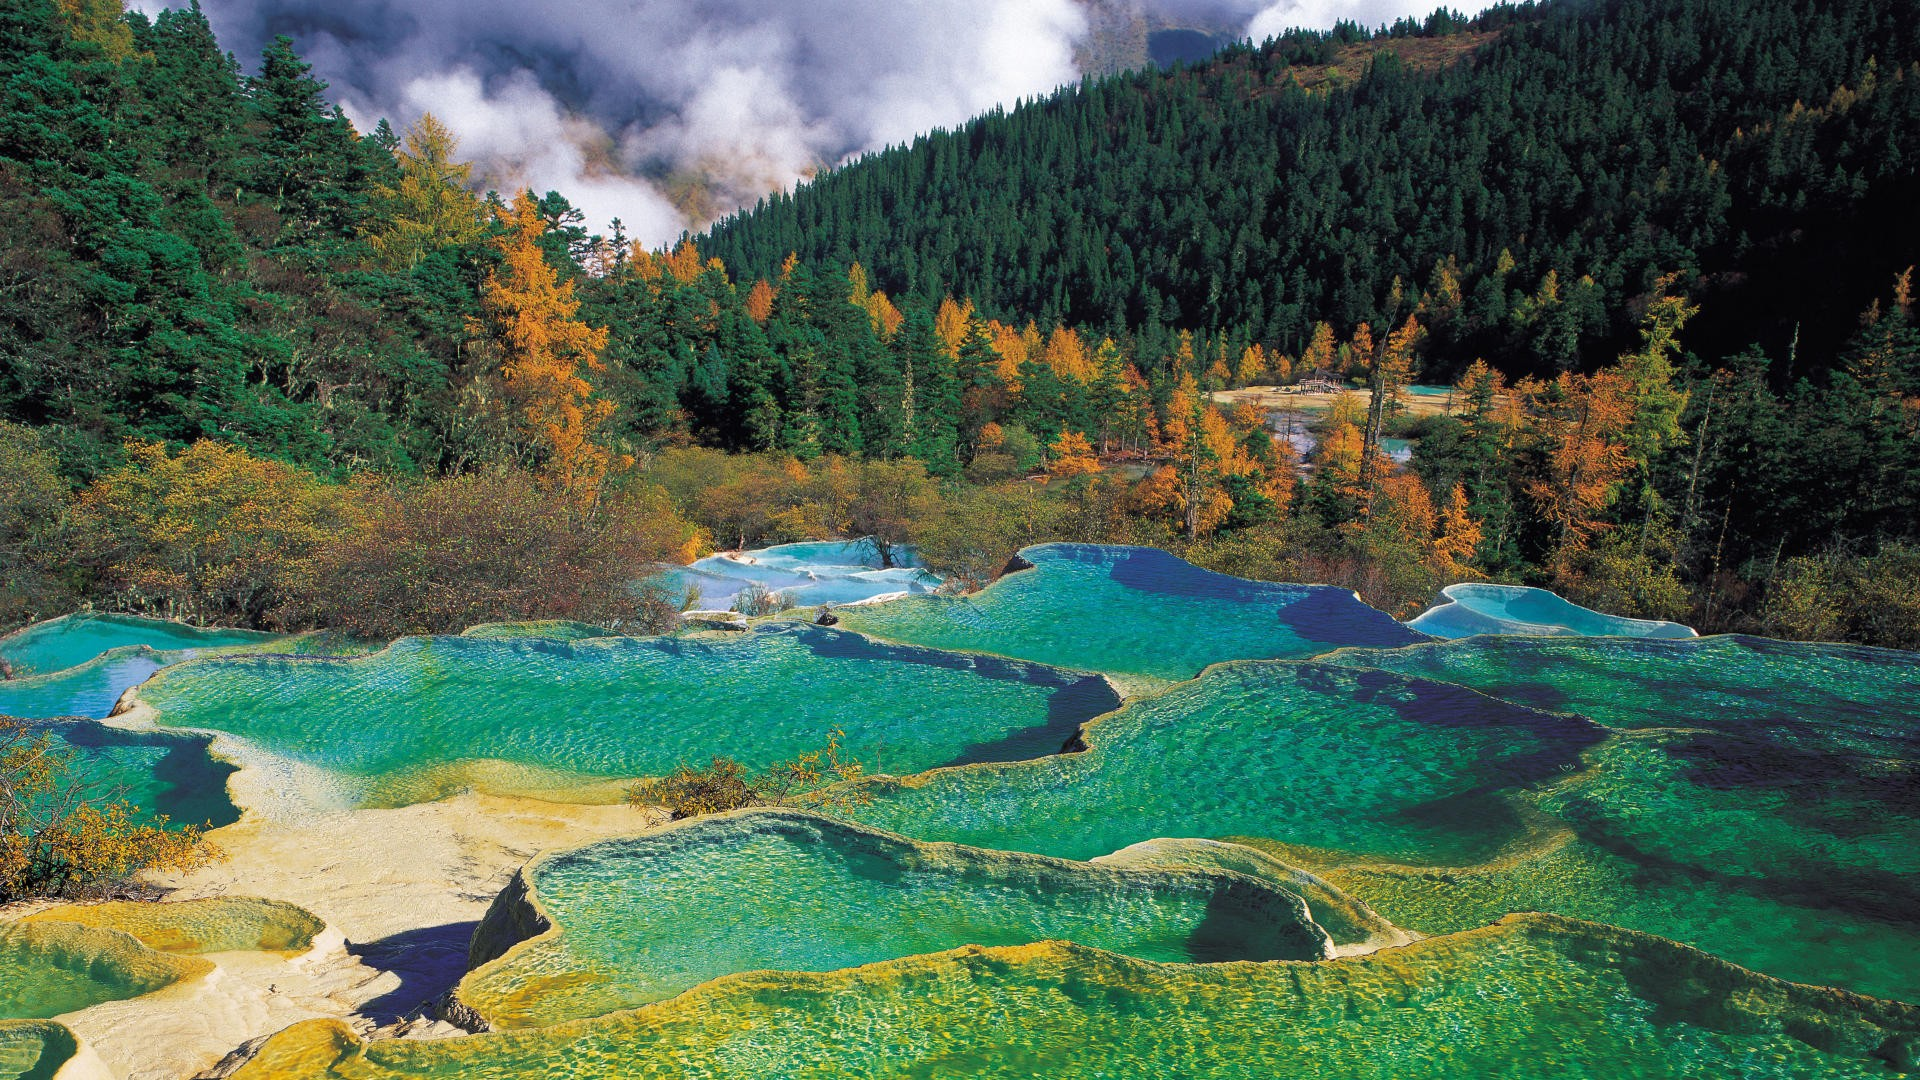
\includegraphics[scale=.15]{pictures/MJzdj.png}
    \caption{Piękny krajobraz}
    \label{fig:a}
    \end{center}
\end{figure}

\subsection{Tabela}
Tabela~\ref{tab:pieniedzy} zawiera informacje na temat wydatków.
\begin{table}[htbt]
\begin{center}
\begin{tabular}{|l|l|l|l|l|}
\hline
\textbf{Imię}       & \textbf{1 dzień} & \textbf{2 dzień} & \textbf{3 dzień} & \textbf{4 dzień} \\ \hline
\textit{Ja}         & 1zł              & 15zł             & 30zł             & 2zł              \\ \hline
\textit{Kolega}     & 40zł             & 10zł             & 20zł             & 30zł             \\ \hline
\textit{Przyjaciel} & 20zł             & 60zł             & 100zł            & 0.5zł            \\ \hline
\textit{Znajomy}    & 80zł             & 10zł             & 60zł             & 99zł             \\ \hline
\end{tabular}
\caption{Wydatki moje i moich kolegów}
\label{tab:pieniedzy}
\end{center}
\end{table}

\newpage
\subsection{Listy numerowane i nie tylko}

\subsubsection{Lista numerowana}
\begin{enumerate}
  \item Item pierwszy
  \item Item drugi
  \item Item trzeci
  \item Item czwarty
\end{enumerate}

\subsubsection{Lista nienumerowana}
\begin{itemize}
  \item Item pierwszy
  \item[\#] Item drugi
  \item[*] Item trzeci
  \item[-] Item czwarty
\end{itemize}

\subsection{2 akapity sformatowanego tekstu}

\noindent {\textbf{Revolutionizing Technology: The Intel 8086 Legacy}}

In the realm of technological innovation, the \textit{Intel 8086} stands as an emblem of transformative brilliance. Like a \textbf{pioneer} mapping uncharted territories, this microprocessor unveiled a new era of computing possibilities. With its \underline{groundbreaking} architecture and visionary design, the \textit{8086} reshaped the landscape of personal computing, laying the cornerstone for modern-day advancements. Its legacy is not merely etched in silicon but \textbf{engraved in the annals of progress}, symbolizing the relentless pursuit of pushing boundaries. From its humble inception, \textbf{it sparked a revolution}, empowering generations of engineers and creators to dream bigger, invent \textbf{bolder}, and sculpt a future fueled by imagination and ingenuity. \\

\noindent {\textbf{Unleashing Potential: Embracing the Intel 8086 Spirit}}

The spirit of the \textit{Intel 8086} resonates beyond its technical specifications; it encapsulates the essence of \textbf{innovation} itself. It teaches us that limitations are mere illusions waiting to be shattered by \underline{perseverance and innovation}. Like the \textit{8086}, we possess the power to redefine possibilities, to \textbf{break free from constraints}, and to chart our course towards \underline{greatness}. Let its story be a beacon, igniting the fire within us to challenge norms, embrace the unknown, and carve our unique imprint on the canvas of \textbf{progress}. Each hurdle is an opportunity, and every setback is a chance to evolve. Let us heed the lessons of this technological marvel and stride forth with unwavering determination, for within each of us lies the \underline{potential to spark the next revolution} and shape the destiny of tomorrow's innovations.